\documentclass[a4paper]{article}

\usepackage[utf8]{inputenc}
\usepackage[margin=0.8in]{geometry}

\usepackage{rotating, graphicx}
\graphicspath{ {../} }
	
\begin{document}


\title{Software Architecture And Design \\ Detecting Code Smells}
\author{Ioan Luca \\ \small 201638554 \\ \small University of Strathclyde}
\date{\today}
\maketitle

\section{Code Smells Overview}
I attempted the ''Middle Man'' code smell from the Hard category,
the ''Long Method'', ''Switch Statements'' and ''Primitive Obsession'' code smells
from the Medium category as well as
the ''Long Class'' and 'Long Parameter List'' from the Easy category.

\subsection{Middle Man}
This code smell happens when a class delegates its responsibility to
another class, usually when attempting to reduce coupling. However, by
doing this, it essentially becomes obsolete.

The software identifies such behaviour by using 2 visitors.
The first one traverses all methods in scope to compile a set of 
method names.
The second visitor identifies methods with a single statement, or with 2
statements
out of which the outer one is a return.
If the statement is a method call that is part of the list, then the smell was
found.

\subsection{Long Method and Long Class}
Long methods/classes are a sign of bad incremental design.
Functionality has been
extended over time without taking into account refactoring.
They are hard to read and they usually break the
''Single responsibility principle''.
The software detects such methods/classes by counting statements inside 
bodies/declarations, including arbitrarily nested statements.
If the number exceeds 10/100, the smell was found.

\subsection{Switch Statements}
Switching on type codes is a bad practice in OOP and it should be handled by
subclassing.
This smell is detected when the expressions being switched on are of
a user defined Enum type.

\subsection{Primitive Obsession}
This appears when sufficiently complex data is handled by primitive types
instead of being abstracted away in a class.
It favours the birth of Data Clumps smells as well.
The software detects this smell inside method and class 
definitions by
counting the total number of variables, parameters and fields.
Afterwards, the primitive declarations are selected from the total and a $ratio$
is calculated with $ratio=\frac{primitives}{total}$.
If $ratio \geq 0.37$ and $primitive \geq 4$ then the code smell was discovered.
The numbers came from trial and error and they appear to discover this
code smell wherever it is present in the testing system.

\subsection{Long Parameter List}
Similar to the Primitive Obsession, having too many parameters breaks both
encapsulation and abstraction.
In addition, it gives a clear clue that the implementation
of a method is quite complex.
The software detects long lists of parameters for both methods and constructors
with more than 5 parameters.

\section{High-level design}

\begin{sidewaysfigure}
	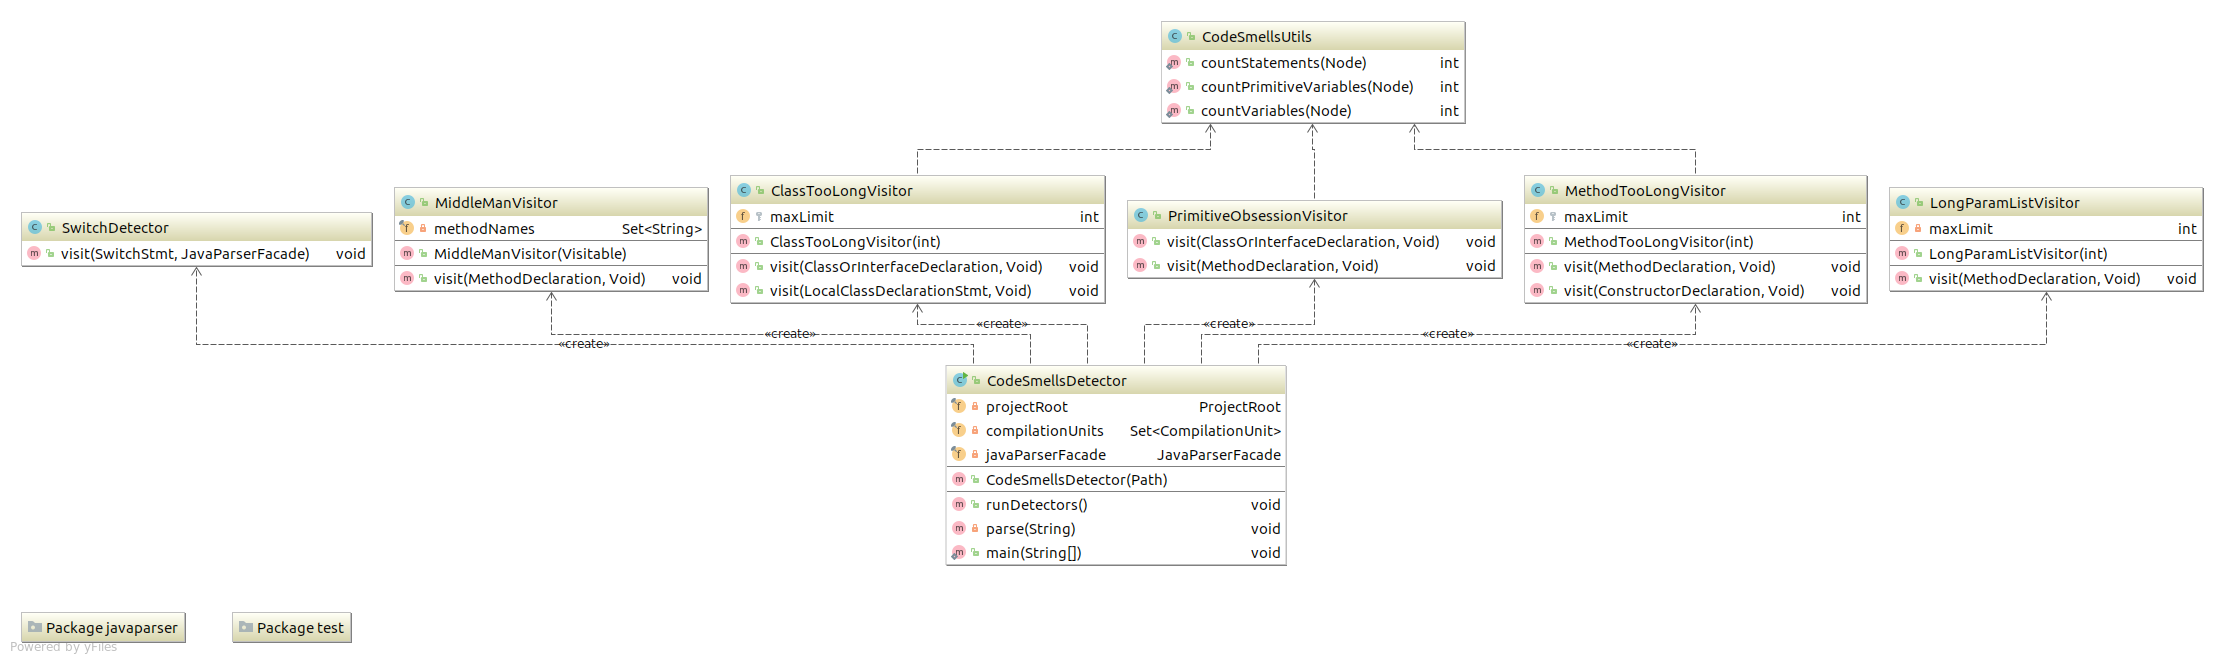
\includegraphics[width=\textwidth]{codesmellspng}
	\caption{Each code smell is implemented using a visitor that extends either
		the generic JavaParser visitor or the the void one.
		The CodeSmellsDetector class is responsible for loading and parsing all
		the sources found in the test system.
		It also runs each visitor on compilation units and
		groups errors by classes.
		Finally, CodeSmellsUtil provides useful functions like counting
		nested statements.}
\end{sidewaysfigure}

Each code smell is implemented using a visitor that extends either
the generic JavaParser visitor or the the void one.

The CodeSmellsDetector class is responsible for loading and parsing all
the sources found in the test system.
It also runs each visitor on compilation units and
groups errors by classes.
Finally, CodeSmellsUtil provides useful functionality like counting
nested statements.

The project was developed using Java 10 and Maven as a build tool plus git for
version control. This report is written in \LaTeX.

Newer versions of JavaParser provide convenience methods to traverse the AST
in a functional style by using the Stream and Map-Reduce APIs.
The source
code tries to use them where possible.

The SwitchDetector is using SymbolParser to test if the type switched on
is an user defined Enum.
SymbolParser is a new addition to JavaParser that implements various 
semantic-driven analyses
based on the AST.

It is worth mentioning that when implementing Primitive Obsession, it is not
enough to check whether a variable declaration is of a primitive type because
the JavaParser method does not check for Strings and other boxed types.
This is acceptable since they are in fact reference types in Java.
The solution considers Strings to be primitives.

The runner class allows to specify a root folder for the Java source files
that need to be analysed and a starting package --- afterwards, it runs
all the smell detectors on each file.

The utility functions use a mix of Map-Reduce and Recursion to traverse the AST.

\section{Results and Evaluation}

The system seems to work reasonably well on the provided test system.
I am not
aware of any false positives. However, there are chances that this software
would fail in more complex cases that I haven't thought about yet.

Moreover, there is uncertainty regarding whether the implementations that work
well for typical method declarations behave the same on lambdas.
They do for anonymous functions.
Similarly, JavaParser has no support for the new $var$ keyword that has recently
been added to Java. Hence, type inference is not as easy when if the source
uses $var$.

\subsection{Program Output}
Below is the output of generated by the program when run on the test system.


\begin{flushleft}
	\subsubsection{in type
		MorpionSolitairePanel-\textgreater{}\textgreater{}}\label{in-type-morpionsolitairepanel-}

	METHOD TOO LONG at mousePressed =\textgreater{} it has 19 which is more
	than 10!

	CONSTRUCTOR TOO LONG at MorpionSolitairePanel =\textgreater{} it has 26
	which is more than 10!

	METHOD TOO LONG at run =\textgreater{} it has 15 which is more than 10!

	METHOD TOO LONG at start =\textgreater{} it has 16 which is more than
	10!

	METHOD TOO LONG at paintComponent =\textgreater{} it has 26 which is
	more than 10!

	SWITCH ON ENUM test.Abusers.Switch.MorpionSolitairePanel.State at
	mousePressed

	MIDDLEMAN at method start

	\subsubsection{in type
		ManOrBoy-\textgreater{}\textgreater{}}\label{in-type-manorboy-}

	LONG PARAMETER LIST at A =\textgreater{} it has 6 which is more than 5!

	\subsubsection{in type Item-\textgreater{}\textgreater{}}\label{in-type-item-}

	PRIMITIVE OBSESSION at CLASS Item --\textgreater{} 4 primitives out of 4
	fields =\textgreater{} that is 100.00 \% primitives

	\subsubsection{in type
		Eertree-\textgreater{}\textgreater{}}\label{in-type-eertree-}

	METHOD TOO LONG at eertree =\textgreater{} it has 28 which is more than
	10!

	PRIMITIVE OBSESSION at METHOD eertree --\textgreater{} 8 primitives out
	of 9 variables =\textgreater{} that is 88.89 \% primitives

	\subsubsection{in type
		BoxingTheCompass-\textgreater{}\textgreater{}}\label{in-type-boxingthecompass-}

	METHOD TOO LONG at main =\textgreater{} it has 13 which is more than 12!

	PRIMITIVE OBSESSION at METHOD buildPoints --\textgreater{} 7 primitives
	out of 7 variables =\textgreater{} that is 100.00 \% primitives

	\subsubsection{in type
		FloodFill-\textgreater{}\textgreater{}}\label{in-type-floodfill-}

	METHOD TOO LONG at floodFill =\textgreater{} it has 26 which is more
	than 10!

	PRIMITIVE OBSESSION at METHOD floodFill --\textgreater{} 8 primitives
	out of 13 variables =\textgreater{} that is 61.54 \% primitives

	\subsubsection{in type Grid-\textgreater{}\textgreater{}}\label{in-type-grid-}

	LONG PARAMETER LIST at checkLine =\textgreater{} it has 6 which is more
	than 5!

	CLASS TOO LONG at Grid =\textgreater{} it has 140 which is more than
	100!

	METHOD TOO LONG at newGame =\textgreater{} it has 12 which is more than
	10!

	METHOD TOO LONG at draw =\textgreater{} it has 36 which is more than 10!

	METHOD TOO LONG at playerMove =\textgreater{} it has 34 which is more
	than 10!

	METHOD TOO LONG at checkLine =\textgreater{} it has 12 which is more
	than 10!

	METHOD TOO LONG at addLine =\textgreater{} it has 11 which is more than
	10!

	PRIMITIVE OBSESSION at METHOD newGame --\textgreater{} 4 primitives out
	of 4 variables =\textgreater{} that is 100.00 \% primitives

	PRIMITIVE OBSESSION at METHOD draw --\textgreater{} 14 primitives out of
	16 variables =\textgreater{} that is 87.50 \% primitives

	PRIMITIVE OBSESSION at METHOD playerMove --\textgreater{} 6 primitives
	out of 13 variables =\textgreater{} that is 46.15 \% primitives

	PRIMITIVE OBSESSION at METHOD checkLine --\textgreater{} 11 primitives
	out of 12 variables =\textgreater{} that is 91.67 \% primitives

	PRIMITIVE OBSESSION at CLASS Grid --\textgreater{} 26 primitives out of
	29 fields =\textgreater{} that is 89.66 \% primitives

	\subsubsection{in type Luhn-\textgreater{}\textgreater{}}\label{in-type-luhn-}

	METHOD TOO LONG at luhnTest =\textgreater{} it has 12 which is more than
	10!

	PRIMITIVE OBSESSION at METHOD luhnTest --\textgreater{} 6 primitives out
	of 6 variables =\textgreater{} that is 100.00 \% primitives

	\subsubsection{in type
		AccountManager-\textgreater{}\textgreater{}}\label{in-type-accountmanager-}

	MIDDLEMAN at method GetAccount

	\subsubsection{in type
		NBodySim-\textgreater{}\textgreater{}}\label{in-type-nbodysim-}

	CONSTRUCTOR TOO LONG at NBody =\textgreater{} it has 23 which is more
	than 10!

	PRIMITIVE OBSESSION at METHOD decompose --\textgreater{} 5 primitives
	out of 5 variables =\textgreater{} that is 100.00 \% primitives

	PRIMITIVE OBSESSION at CLASS NBody --\textgreater{} 4 primitives out of
	7 fields =\textgreater{} that is 57.14 \% primitives

	\subsubsection{in type
		CipollasAlgorithm-\textgreater{}\textgreater{}}\label{in-type-cipollasalgorithm-}

	METHOD TOO LONG at c =\textgreater{} it has 29 which is more than 10!

	\subsubsection{in type
		BresenhamPanel-\textgreater{}\textgreater{}}\label{in-type-bresenhampanel-}

	METHOD TOO LONG at paintComponent =\textgreater{} it has 15 which is
	more than 10!

	METHOD TOO LONG at drawLine =\textgreater{} it has 28 which is more than
	10!

	PRIMITIVE OBSESSION at METHOD paintComponent --\textgreater{} 12
	primitives out of 13 variables =\textgreater{} that is 92.31 \%
	primitives

	PRIMITIVE OBSESSION at METHOD plot --\textgreater{} 10 primitives out of
	11 variables =\textgreater{} that is 90.91 \% primitives

	PRIMITIVE OBSESSION at METHOD drawLine --\textgreater{} 13 primitives
	out of 14 variables =\textgreater{} that is 92.86 \% primitives

	\subsubsection{in type
		HuffmanCode-\textgreater{}\textgreater{}}\label{in-type-huffmancode-}

	METHOD TOO LONG at printCodes =\textgreater{} it has 12 which is more
	than 10!

	\subsubsection{in type
		BarnsleyFern-\textgreater{}\textgreater{}}\label{in-type-barnsleyfern-}

	METHOD TOO LONG at createFern =\textgreater{} it has 19 which is more
	than 10!

	PRIMITIVE OBSESSION at METHOD createFern --\textgreater{} 8 primitives
	out of 8 variables =\textgreater{} that is 100.00 \% primitives

	\subsubsection{in type
		Client-\textgreater{}\textgreater{}}\label{in-type-client-}

	MIDDLEMAN at method something

	MIDDLEMAN at method somethingElse

	\subsubsection{in type
		BarnsleyFernTwo-\textgreater{}\textgreater{}}\label{in-type-barnsleyferntwo-}

	METHOD TOO LONG at createFernWithTemp =\textgreater{} it has 18 which is
	more than 10!

	PRIMITIVE OBSESSION at METHOD createFernWithTemp --\textgreater{} 6
	primitives out of 6 variables =\textgreater{} that is 100.00 \%
	primitives

	\subsubsection{in type Test-\textgreater{}\textgreater{}}\label{in-type-test-}

	PRIMITIVE OBSESSION at METHOD meanStdDev --\textgreater{} 4 primitives
	out of 5 variables =\textgreater{} that is 80.00 \% primitives

	PRIMITIVE OBSESSION at METHOD showHistogram01 --\textgreater{} 5
	primitives out of 6 variables =\textgreater{} that is 83.33 \%
	primitives

	PRIMITIVE OBSESSION at CLASS Test --\textgreater{} 4 primitives out of 4
	fields =\textgreater{} that is 100.00 \% primitives

\end{flushleft}

\end{document}
